% vim:ts=4:sw=4
% Copyright (c) 2014 Casper Ti. Vector
% Public domain.

\chapter{系统实现}
\section{爬虫模块}
基于在本文第二部分中的数据来源和爬虫的分析,采用beautifulSoup技术来进行扒取数据。
\subsection{爬取基本数据}
\begin{figure}[h]
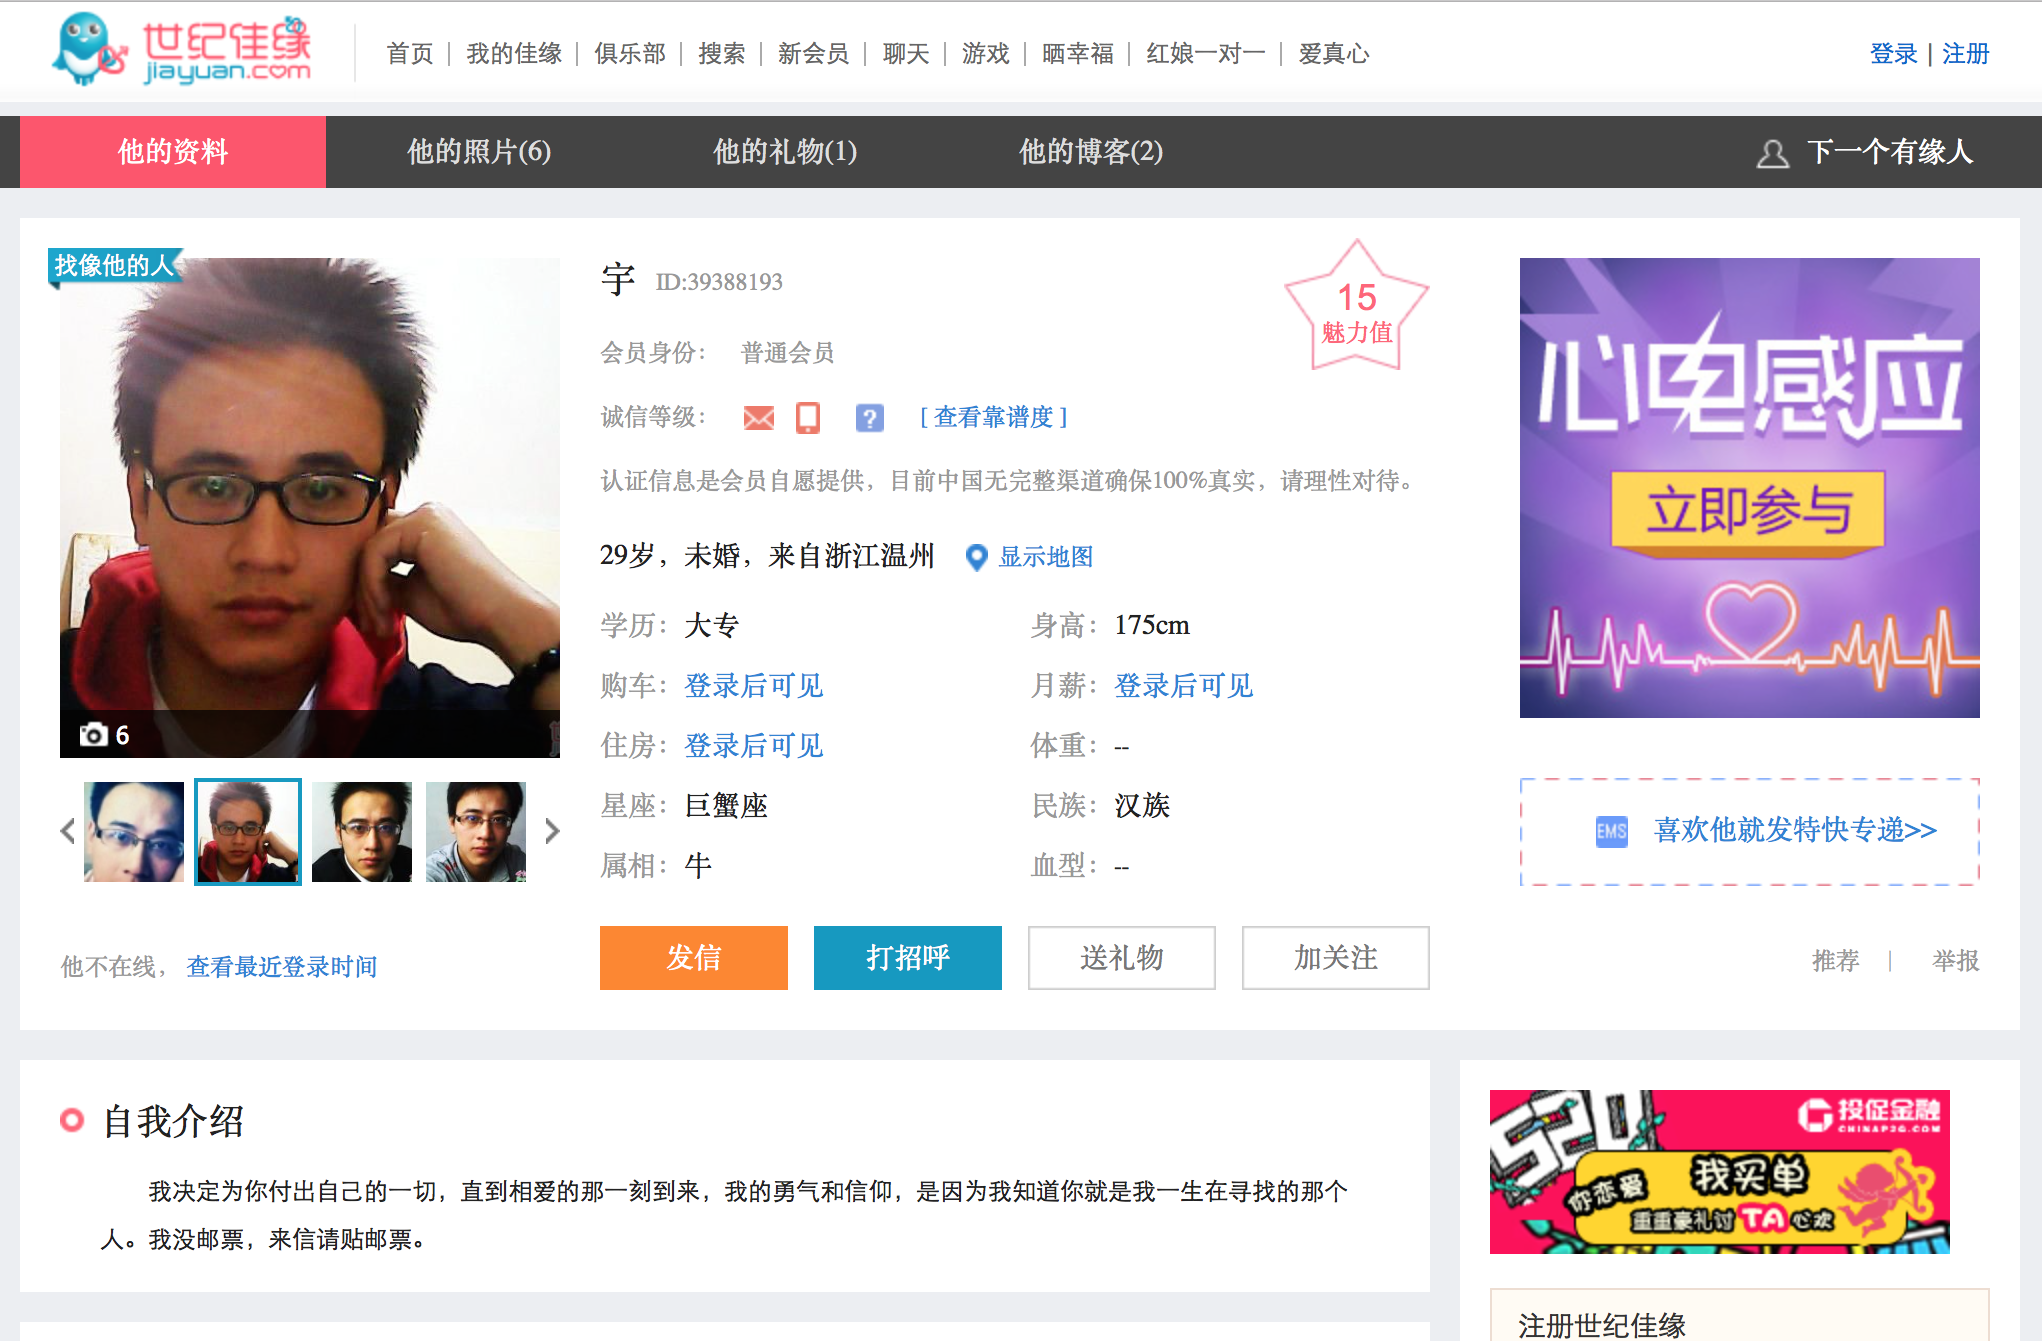
\includegraphics[width=\textwidth]{img/chap4/jiayuan1.png}
\caption{世纪佳缘用户信息页面\label{Face++API}}
\end{figure}
\begin{figure}[h]
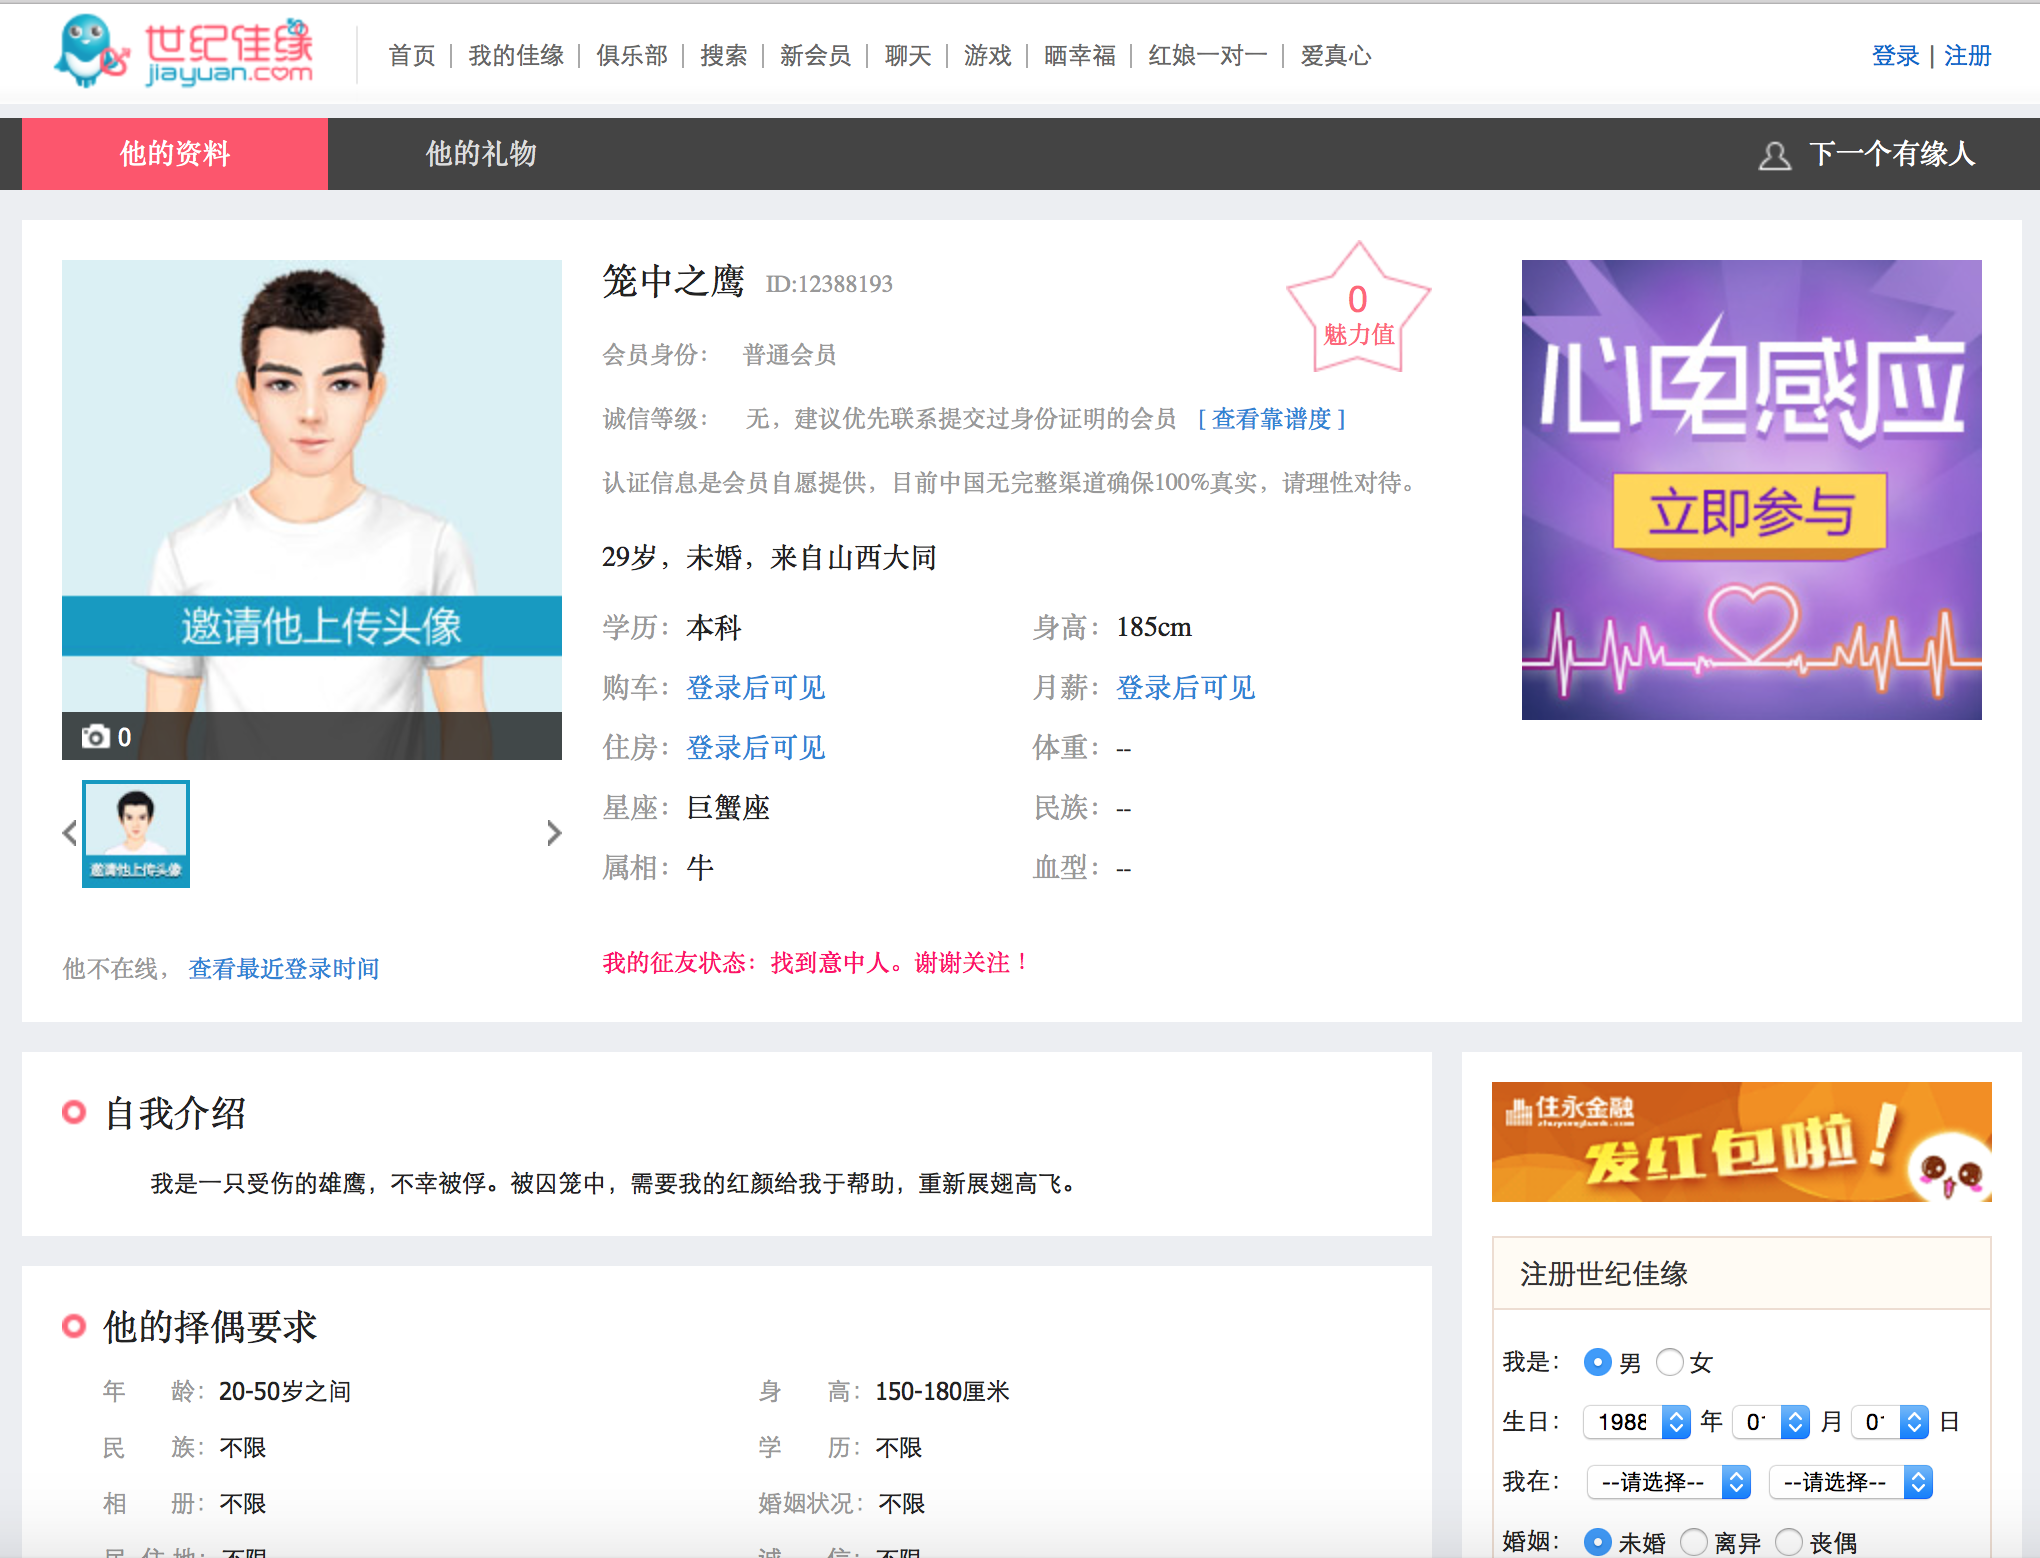
\includegraphics[width=\textwidth]{img/chap4/jiayuan2.png}
\caption{世纪佳缘需权限信息页面\label{Face++API}}
\end{figure}

通过前期充分对于世纪佳缘网站上数据的发掘,本文找到了一个基于用户id以及对应用户数据的网页,从图4.1,图4.2可以看出,此网页url为用户id与前缀结合,而除了一些用户的图片和信息设置为成权限可见之外,其他的数据对于爬虫都是友好的。最后对于抓取到的数据信息,存储到到用户数据库之中。伪代码如下所示。

\begin{codebox}
\Procname{$\proc{Crawler}$}
\li \For $j \gets $ \To the Amount of extrace \label{li:for}
\li     \Do \label{li:for-begin}
\li 	$Data \gets$ info from url
\li \For $k \gets$ Every Elements form $Data$\label{li:for}
\li     \Do \label{li:for-begin}
\li      Insert $k$ into the sorted sequence $Request$.
\label{li:for-end}
                \End
\li         $Request$ submit to database       \label{li:for-end}
        \End
\end{codebox}

% [伪代码1]
% \subsection{导入数据库}

% [伪代码2]

\section{应用端模块}
该应用的实现由三步组成:状态查询,信息源添加,和匹配反馈。
具体的应用端的逻辑,由一个类似的iOS框架图来类比。

\subsection{状态查询及展示}
为了满足用户自己查询感兴趣好友的需求,应用需要提供用户在使⽤应⽤程序查看他人已经存在的用户信息。并为了便携性和可用性,需完成进行对于用户信息的一个预览,以及对于具体应用信息的查询。

从而可以满足用户的需求,去其他用户查看具体的信息,并可以支持用户随时对于需要的信息的刷新,以及链接用户更进一步的个人主页的途径。
\begin{figure}[h] 
\begin{minipage}[t]{0.3\linewidth}
\centering
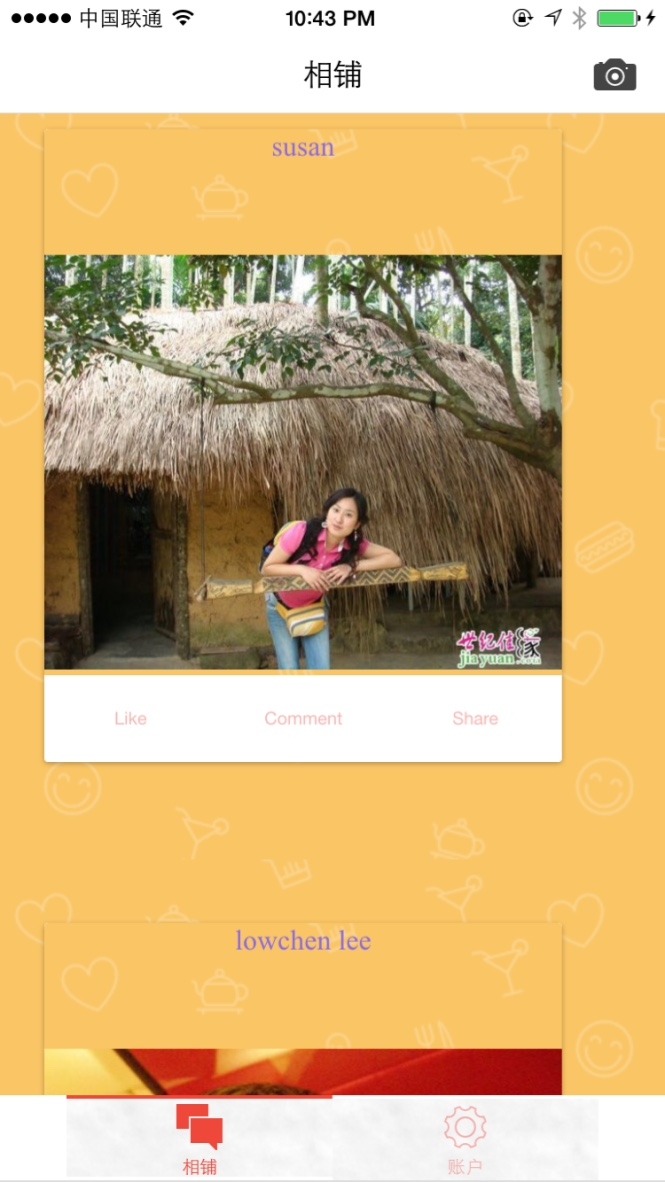
\includegraphics[width=\textwidth]{img/chap4/info1.jpg}
\caption{主界面\label{flickr}}
\end{minipage}
\hfill
\begin{minipage}[t]{0.3\linewidth}
\centering
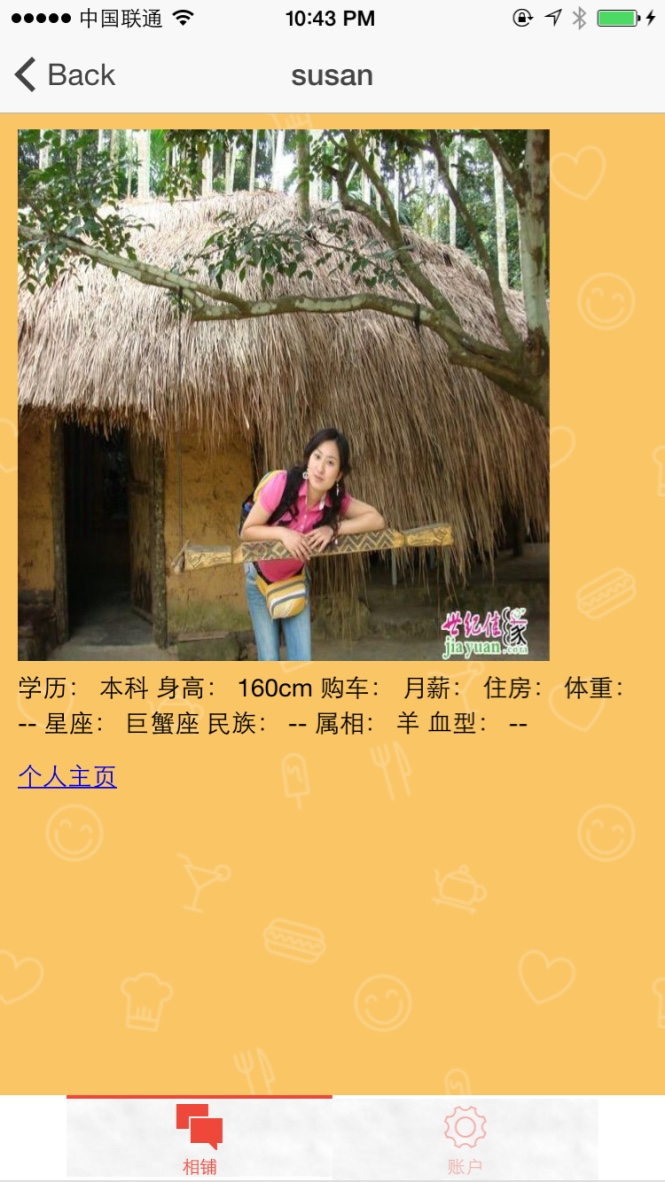
\includegraphics[width=\textwidth]{img/chap4/info2.jpg}
\caption{详细信息\label{instagram}}
\end{minipage}
\hfill
\begin{minipage}[t]{0.3\linewidth}
\centering
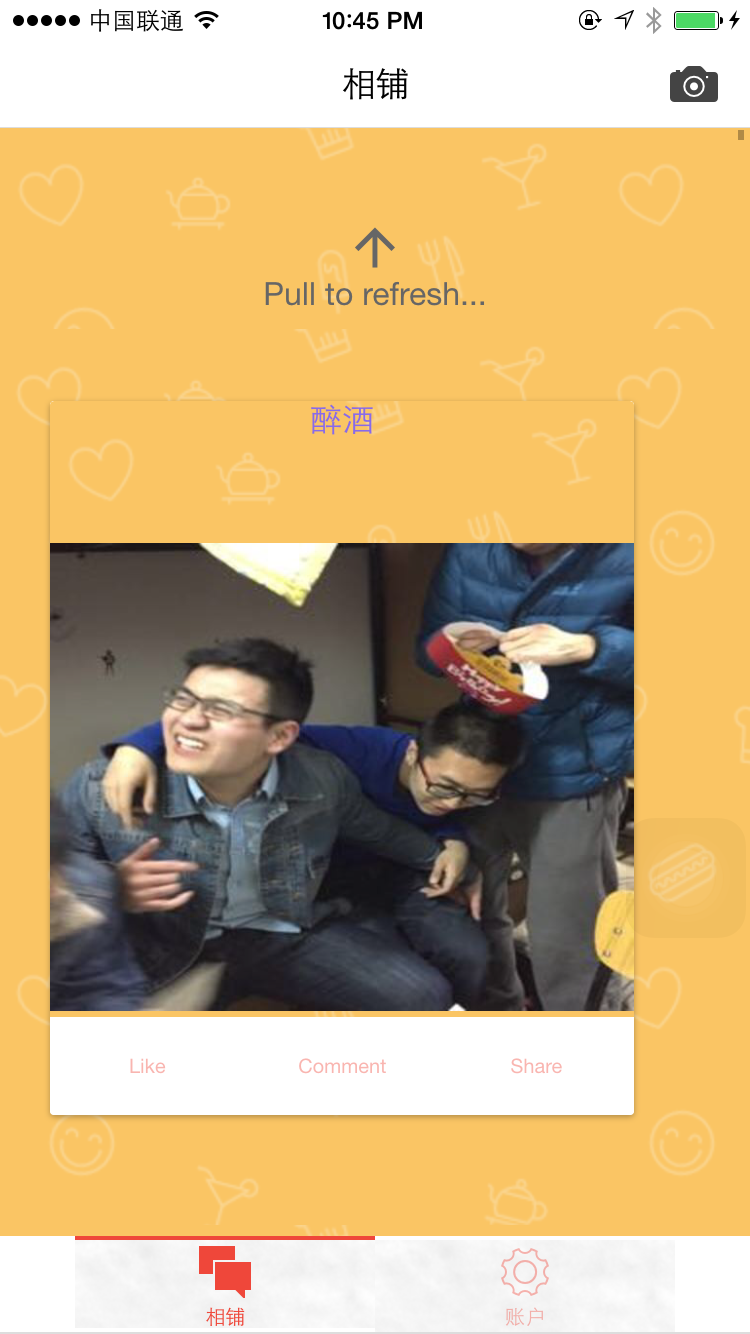
\includegraphics[width=\textwidth]{img/chap4/info3.PNG}
\caption{刷新\label{snapchat}}
\end{minipage}
\hfill
\end{figure}

\subsection{信息源添加}
用户关系自己信息的发布通常希望其发布的信息具有多种多样的形式,考虑到移动设备较难编辑和显⽰示富⽂文本信息,应⽤用程序被实现为能够编辑、存储和显⽰示具有多种类型的字段,包括个人姓名、个人介绍、URL和提交的匹配图片

并且基于用户照片来源的不同,分为从用户的图片库中采集和及时照相功能。并在此基础上实现了图片预览的功能
\begin{figure}[h] 
\begin{minipage}[t]{0.45\linewidth}
\centering
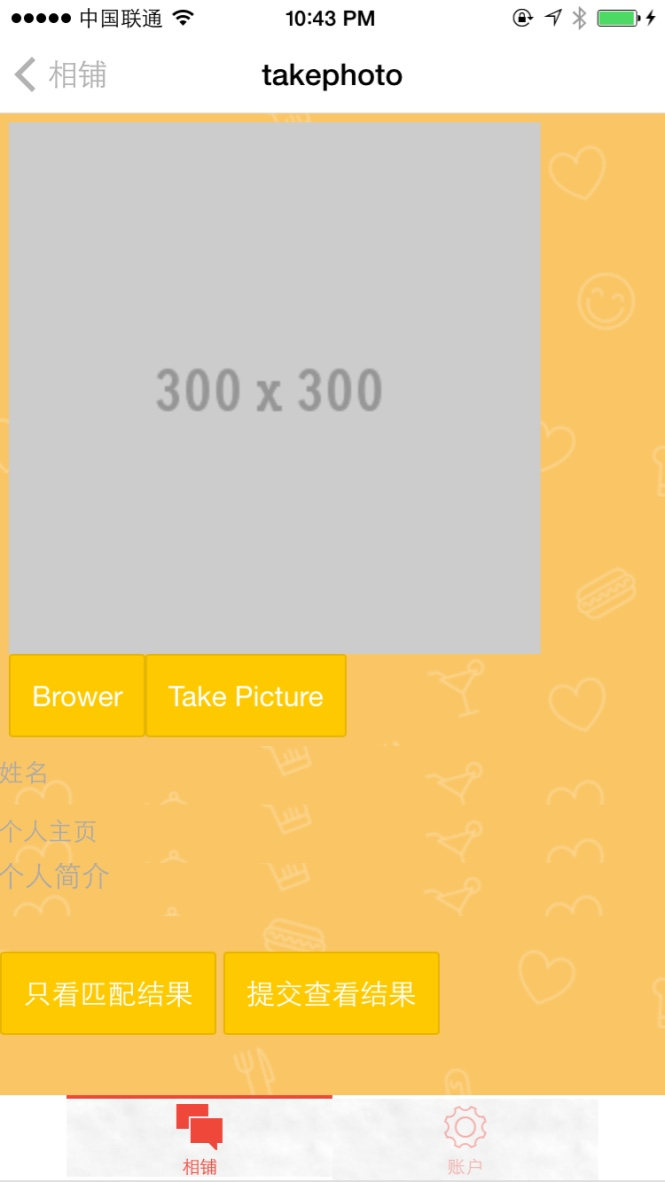
\includegraphics[width=\textwidth]{img/chap4/take1.jpg}
\caption{主界面\label{flickr}}
\end{minipage}
\hfill
\begin{minipage}[t]{0.45\linewidth}
\centering
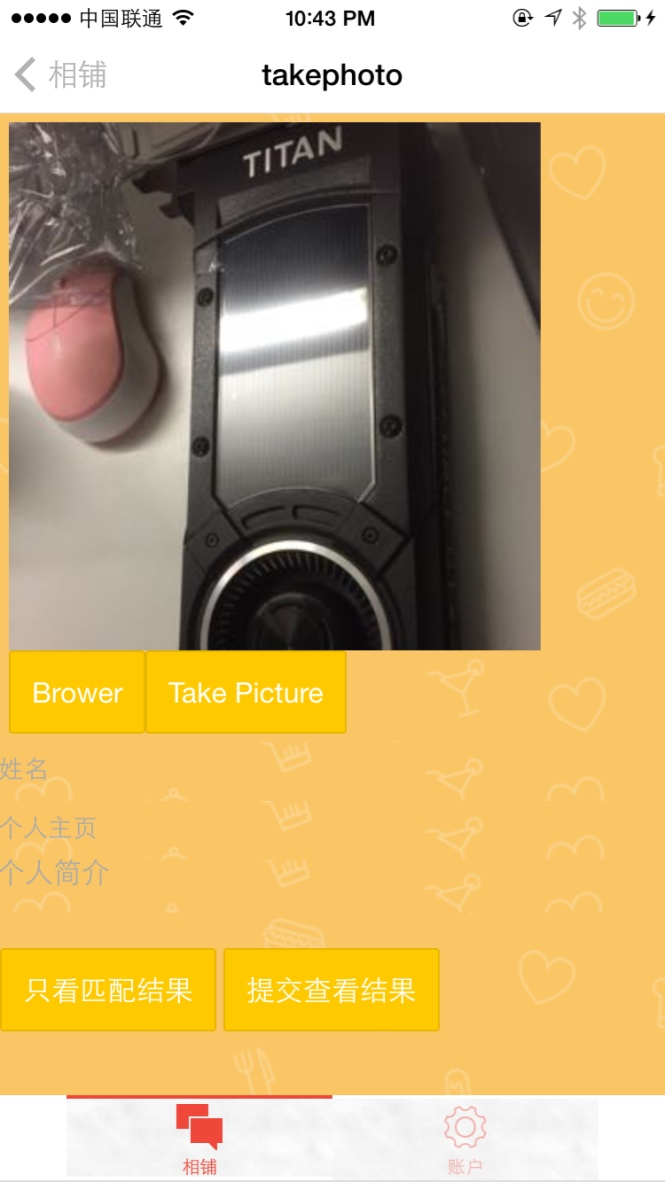
\includegraphics[width=\textwidth]{img/chap4/take2.jpg}
\caption{详细信息\label{instagram}}
\end{minipage}


\end{figure}
\subsection{匹配信息展⽰}
由于服务端有客户端提交的图片以及文本信息直接调用对应匹配算法的接口,因此,应用端在用户在提交了自己的信息之后便直接调用了此接口,服务端便具有了足够的信息以匹配出对应的好友。

在服务端返回给客户端匹配出的结果后,客户端将详细信息显⽰示在⽤用户界⾯面上。这里具有具有多条匹配结果,客户端将按照匹配程度顺序将结果显⽰。当用户对该用户感兴趣时即点击按钮进入查询详细信息。

\begin{figure}[h] 
\begin{minipage}[t]{0.45\linewidth}
\centering
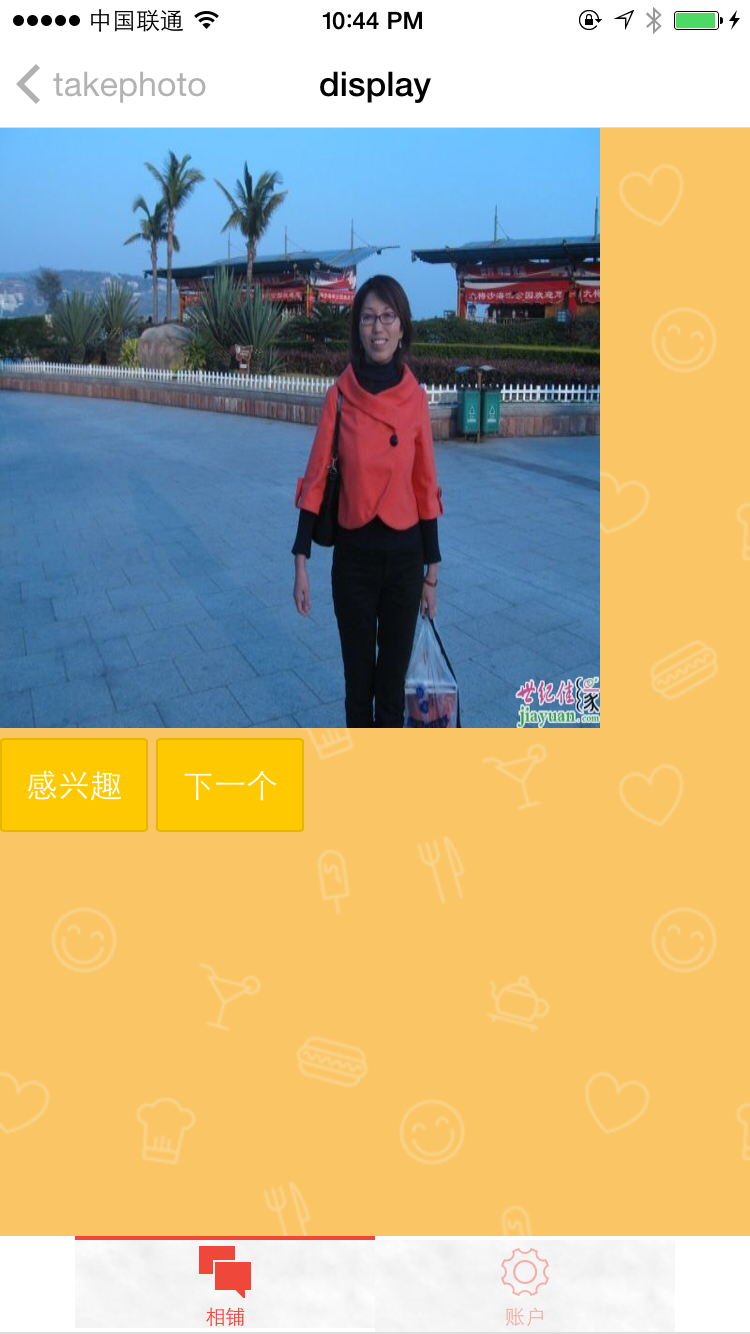
\includegraphics[width=\textwidth]{img/chap4/display.PNG}
\caption{展示界面\label{instagram}}
\end{minipage}


\end{figure}

% 中文测试文字。


